% !TeX root = ../Notizen.tex

\section*{Aufgabe 4: Kepler-Ellipsen}
Das Programm aus Aufgabe 1 wird jetzt verwendet, um die Planetenbahnen zu bestimmen.
Dazu wird die Zentralkraft verwendet
\begin{align}
	\frac{1}{m}\vec{F}(\vec{r})=-G\frac{\vec{r}}{r^3}~,
\end{align}
wobei $G=1$ gesetzt wird.
\subsection*{a)}
Hier werden zwei Teilchenbahnen für die Masse $m=\SI{1}{kg}$ erstellt.
Für das erste Teilchen werden die Startvektoren 
\begin{align}
	\vec{r}_1=
	\begin{pmatrix}
		1,0\\0,0\\0,0
	\end{pmatrix}\text{ und }
	\vec{v}_1=
	\begin{pmatrix}
		-0,5\\1,0\\0,0
	\end{pmatrix}
\end{align}
verwendet und für den zweiten
\begin{align}
	\vec{r}_2=
	\begin{pmatrix}
		1,0\\0,0\\0,0
	\end{pmatrix}\text{ und }
	\vec{v}_2=
	\begin{pmatrix}
		-0,1\\1,0\\0,0
	\end{pmatrix}.
\end{align}
Die resultierenden Bahnen sind in \cref{fig:Bahn} dargestellt.
Diese wurden mit $h=0,01$ und $t=\SI{10}{s}$ erstellt.
In \cref{fig:Bahn2} ist die Bahn für größere Breiten dargestellt.
Es lässt sich erkennen, dass die Ellipse erst eckiger wird und sich später wie eine Spirale zum Ursprung bewegt.
Für kleine Anfangsgeschwindigkeiten fällt das Teilchen in den Ursprung und bekommt eine starke Beschleunigung und läuft dann weg, wie in \cref{fig:Bahn3} dargestellt.\\

\begin{figure}[H]
	\begin{subfigure}[c]{0.5\textwidth}
		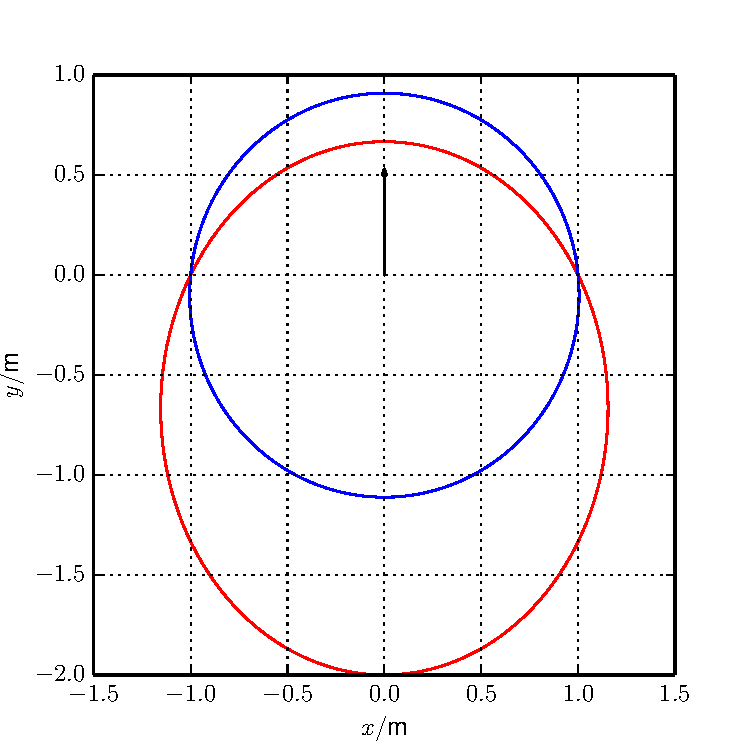
\includegraphics[width = \textwidth]{../Plots/Plot_4_A_1.pdf}
		\caption{2 simulierte Planetenbahnen sowie der Lenz-Runge-Vektor.\label{fig:Bahn}}
	\end{subfigure}
	\begin{subfigure}[c]{0.5\textwidth}
		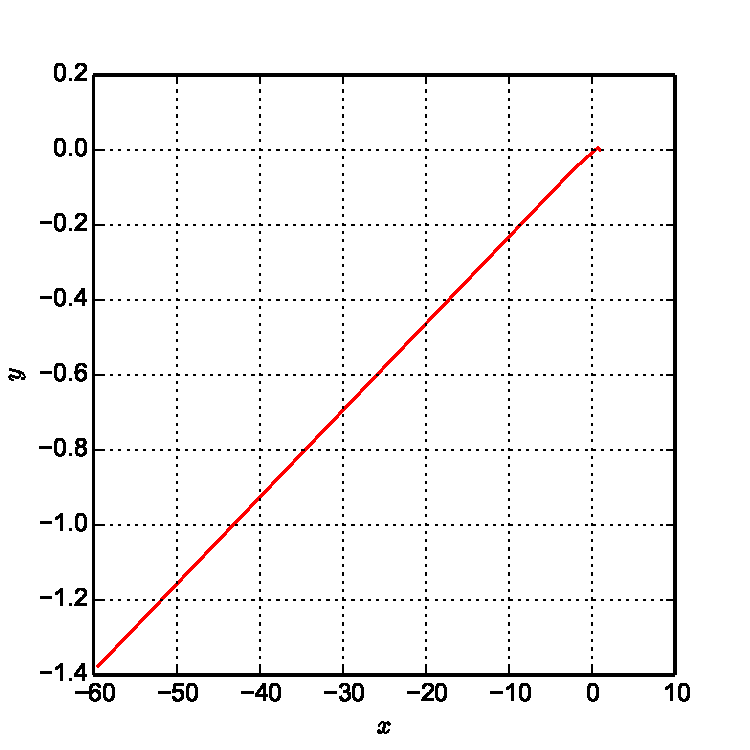
\includegraphics[width = \textwidth]{../Plots/Plot_4_A_5.pdf}
		\caption{Verhalten der Planetenbahn für kleine Anfangsgeschwindigkeiten. \label{fig:Bahn3}}
	\end{subfigure}
	\begin{subfigure}[c]{0.5\textwidth}
		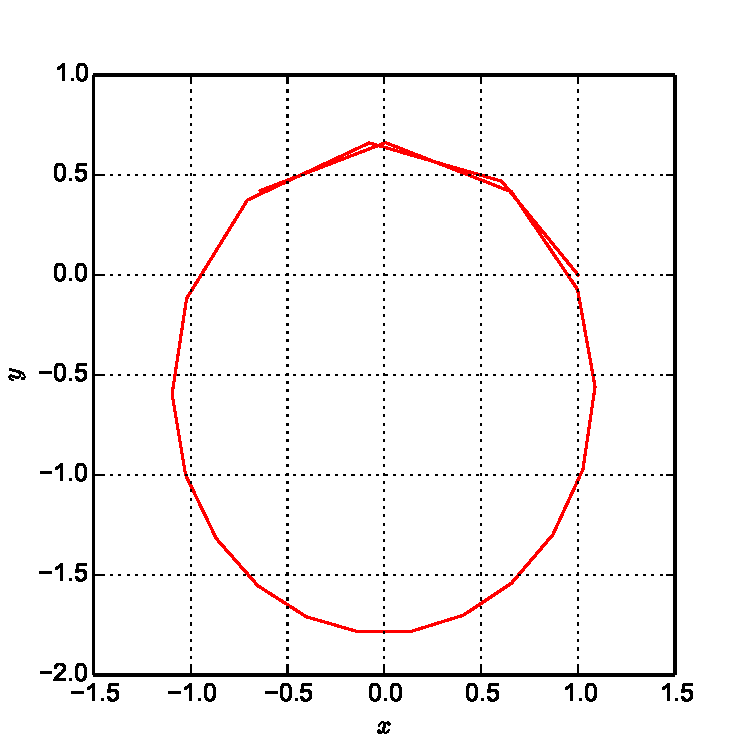
\includegraphics[width = \textwidth]{../Plots/Plot_4_A_3.pdf}
		\caption{Planetenbahn für $h=0,5$.}
	\end{subfigure}
	\begin{subfigure}[c]{0.5\textwidth}	
		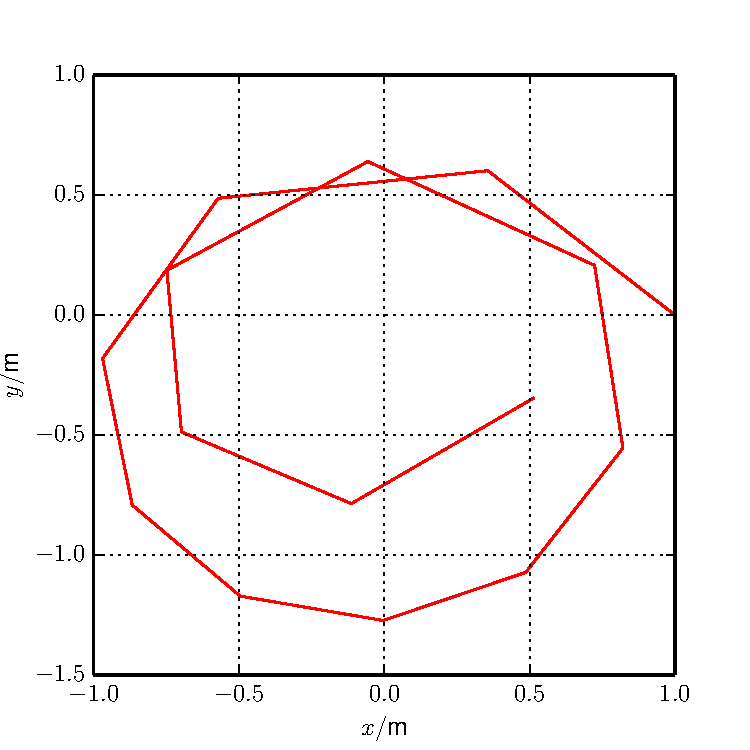
\includegraphics[width = \textwidth]{../Plots/Plot_4_A_4.pdf}
		\caption{Planetenbahn für $h=0,7$.\label{fig:Bahn2}}
	\end{subfigure}\\
\end{figure}
\subsection*{b)}
Als nächstes soll überprüft werden, ob die Energie in dem System erhalten ist.
Sie ist definiert als
\begin{align}
	E:=\frac{1}{2}v^2-\frac{mG}{r}
\end{align}
Hier wird wieder die Energiedifferenz $\Delta E$ für unterschiedliche Zeiten $t$ betrachtet.
Aus ihrer Größenordnung von $e-6$ ist ersichtlich, dass die Energie wieder im Wesentlichen erhalten ist.
\begin{figure}[H]
	\centering
	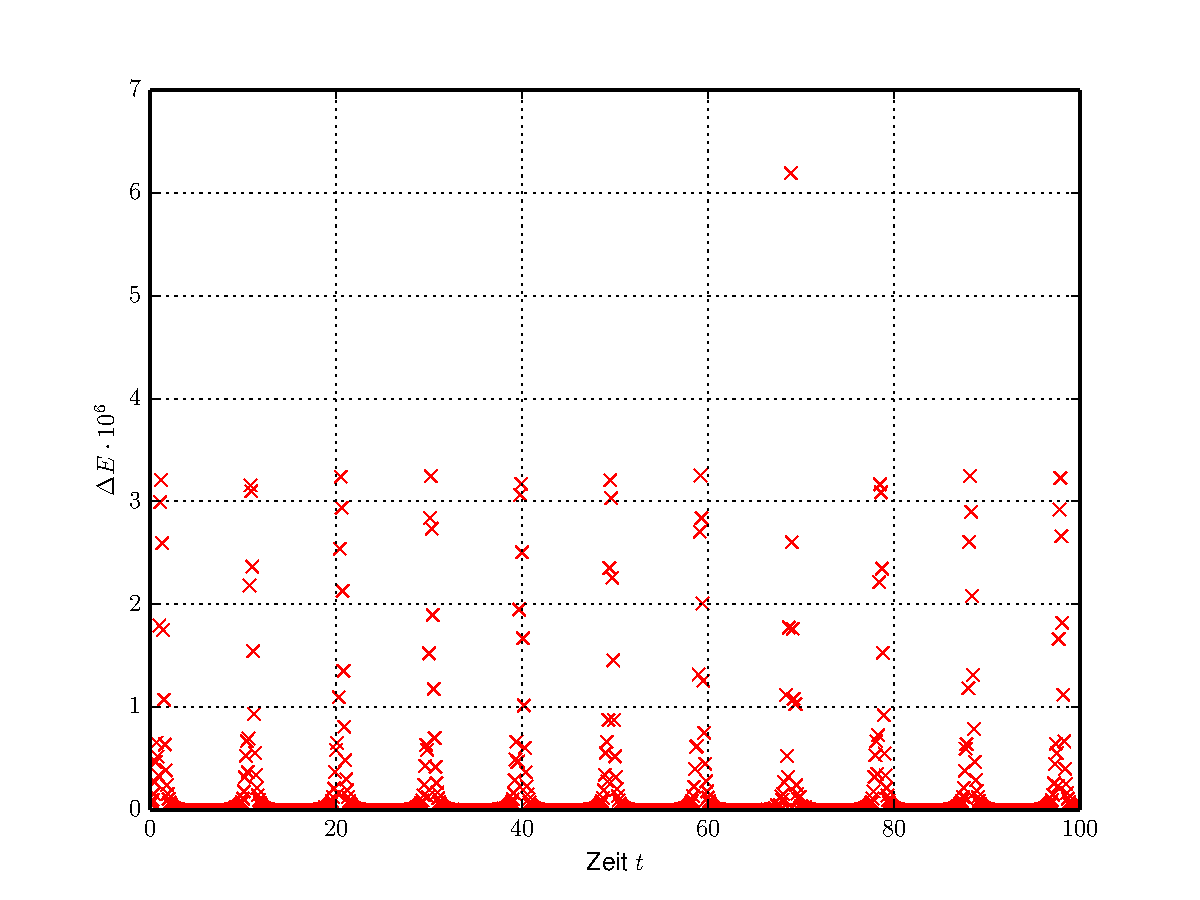
\includegraphics[width = \textwidth]{../Plots/Plot_4_Energie.pdf}
	\caption{Energiedifferenz $\Delta E$ für verschiedene Zeiten $t$.\label{fig:Energie}}
\end{figure}
